\section{Results}
\label{sec:results}

We first explored the difference in performance between Morton and Hilbert keys. We also explored the execution time of an initial build versus the subsequent perturbation rebalance. We broke down the construction time into the high level algorithm components, to gather metrics of interest for further profiling at the system and kernel level in the second half of the project and to guide any optimization efforts.

\subsection{Bottleneck}

A general test to develop a sense of Cornerstone's internal bottlenecks is done on a single GPU comparing a case with 100 million particles using either Hilbert or Morton keys. The test loop contains the code to compute the SFC, do a radix sort, reorder the corresponding particle properties, and update the leaves and then internal tree state; these are the steps needed to compute the octree and have it in a usable state. Immediately we see that the sorting and reordering of particle properties is very dominant in this regime. Therefore, these kernels will be the main target of optimizations, which will be covered in the latter stages of this project.

\begin{figure}[h!]
    \centering
    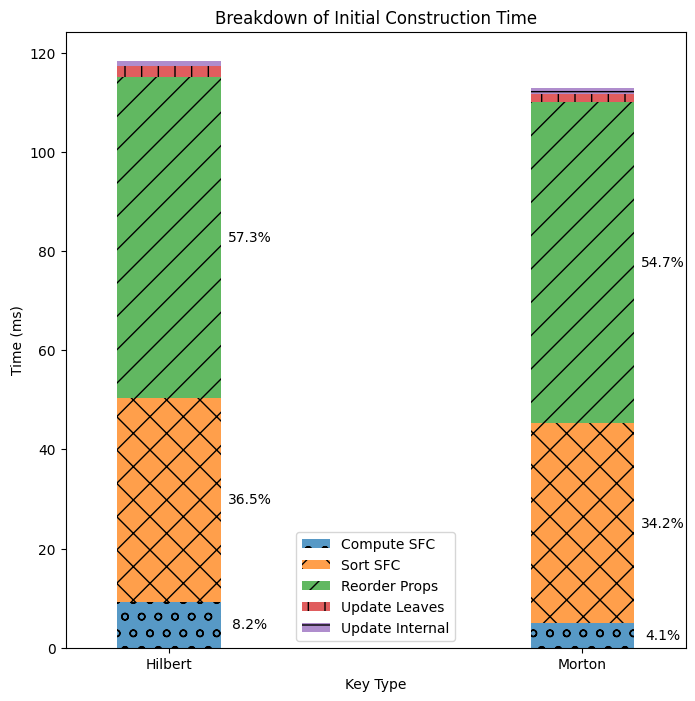
\includegraphics[width=0.45\textwidth]{assets/init_100m.png}
    \caption{Comparison of operations in a broader tree update on a single GPU.}
    \label{fig:keys_100m}
\end{figure}

Figure \ref{fig:keys_100m} breaks down the runtime of both the Hilbert and Morton key cases using the local only build with 100 million particles. The dominant factor in the calculation is the reordering and sorting of the keys and corresponding particles with the actual building of the tree and computation of the space filling curves taking only $\approx 10\%$ of the total build time. This is to be expected, as we mention in \ref{sec:cornerstone}, computation of SFCs for particles and the subsequent sorting and reordering operates on the total number of particles which is typically much greater than the number of nodes in the octree assuming $N_{crit}$ is greater than 1, so the first part of the build has more work to do. This aligns with results from Keller et al. ~\cite{cornerstone} when they profile Cornerstone, their A100 profile is given below. The benchmark from their paper matches our breakdown here with Radix sort dominating although they do not consider the time to do gather's of particle properties to match the new layout.

\begin{table}[h]
\centering
\caption{Original Cornerstone profile on an A100 GPU, adapted from ~\cite{cornerstone}.}
\begin{tabular}{||c c c c||} 
 \hline
 execution on A100 & 1M & 32M & 512M \\ [0.5ex] 
 \hline\hline
 64-bit Morton keys & 0.018 ms & 0.31 ms & 7.9 ms \\ 
 \hline
 64-bit Hilbert keys & 0.084 ms & 1.9 ms & 30 ms \\
 \hline
 Radix sort & 0.483 ms & 5.0 ms & 73 ms \\
 \hline
 Leaf Update & 0.11 ms & 0.51 ms & 2.5 ms \\
 \hline
 Interal Nodes & 0.19 ms & 0.65 ms & 5.4 ms \\ [1ex] 
 \hline
\end{tabular}
\end{table}

\subsection{Initial Distributions}

Focusing on overall runtime, there is a stark distinction of behavior between low particle count (1 million and less) and high particle count (10 million and more) workloads. The runtime of low particle workloads either is not significantly impacted by the initial distribution, as shown in Figure \ref{fig:gist_10k} or behaves unpredictably as shown in Figure \ref{fig:gist_100k}. A consistent pattern emerges across high particle workloads, which is shown in Figure \ref{fig:gist_100m}. Here we can see that, generally, lower dimension manifolds have lower construction cost associated with them.

There is no consistently worst or best initial distribution as can be gleamed in figures \ref{fig:gist_10k}, \ref{fig:gist_100k}, and \ref{fig:gist_100m}. This is somewhat surprising, the author of Cornerstone, Keller mentioned that filaments and pancakes were difficult distributions for Cornerstone to process efficiently due to the large amounts of space that may be wasted in dividing the octants.

\begin{figure}[h!]
    \centering
    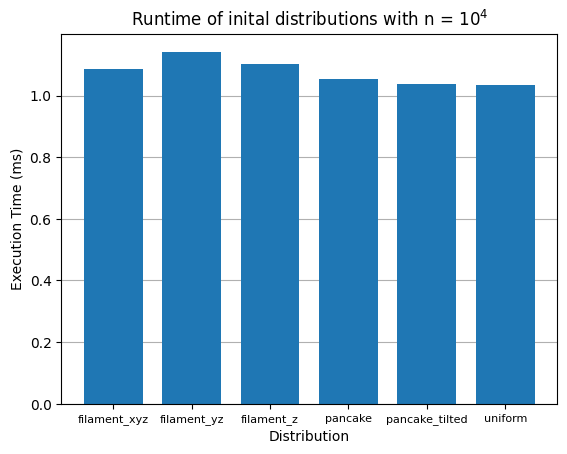
\includegraphics[width=0.45\textwidth]{assets/gist_n10k.png}
    \caption{Construction time of different initial distributions for a low particle workload of n = $10^4$.}
    \label{fig:gist_10k}
\end{figure}

\begin{figure}[h!]
    \centering
    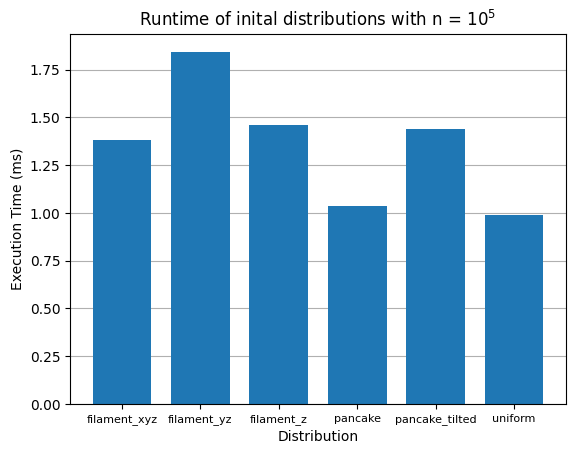
\includegraphics[width=0.45\textwidth]{assets/gist_n100k.png}
    \caption{Construction time of different initial distributions for a low particle workload of n = $10^5$.}
    \label{fig:gist_100k}
\end{figure}

\begin{figure}[h!]
    \centering
    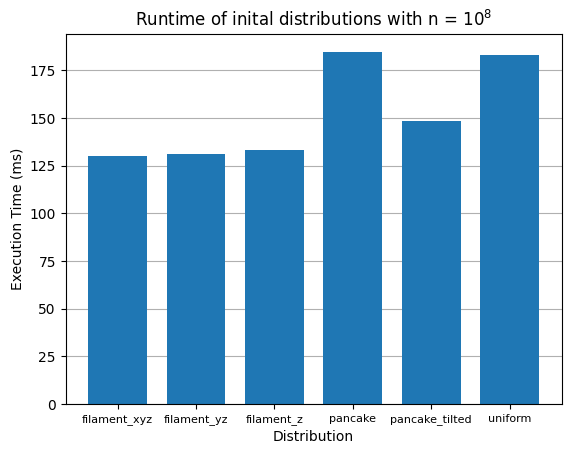
\includegraphics[width=0.45\textwidth]{assets/gist_n100m.png}
    \caption{Construction time of different initial distributions for a high particle workload of n = $10^8$.}
    \label{fig:gist_100m}
\end{figure}

\subsection{Perturbations}

To analyze the effects of perturbations, the update time of the octree after a perturbation is applied was compared to the initial construction time octree for each distribution. It is clear that, for the low particle workloads, perturbations have very little impact on update time as shown in Figure \ref{fig:plot_10k}. Only for high particle workloads does the correlation of perturbation strength to relative update speed become noticeable, as shown in Figure \ref{fig:plot_100m}.

The perturbations have varying effectiveness depending on the initial distribution to which they are applied. This is likely due to the fact that the initial distributions are easily expressed by the octree, which applying a perturbation degrades. This is bolstered by the fact that the distributions which are most susceptible to perturbations are also the ones that have the lowest initial construction time. This is likely why the uniform distribution is not affected greatly by perturbations until a perturbation level of .5, when the filament distributions see a steady performance decrease at increasing perturbation levels. It is important to note that a relative execution time greater than 100\% does not mean updating the octree is slower than reconstructing it from scratch as the perturbed distribution may still take longer to generate from scratch. 

\begin{figure}[h!]
    \centering
    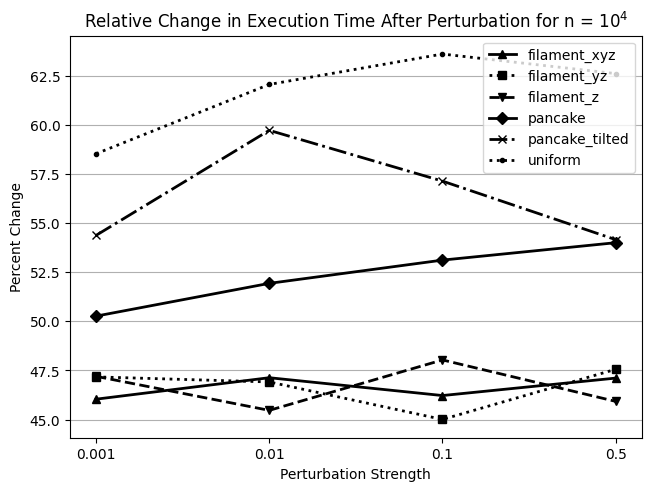
\includegraphics[width=0.45\textwidth]{assets/plotted_n10k.png}
    \caption{Perturbed octree rebalancing time relative to initial build time for different perturbation strengths for a low particle workload of n = $10^4$.}
    \label{fig:plot_10k}
\end{figure}

\begin{figure}[h!]
    \centering
    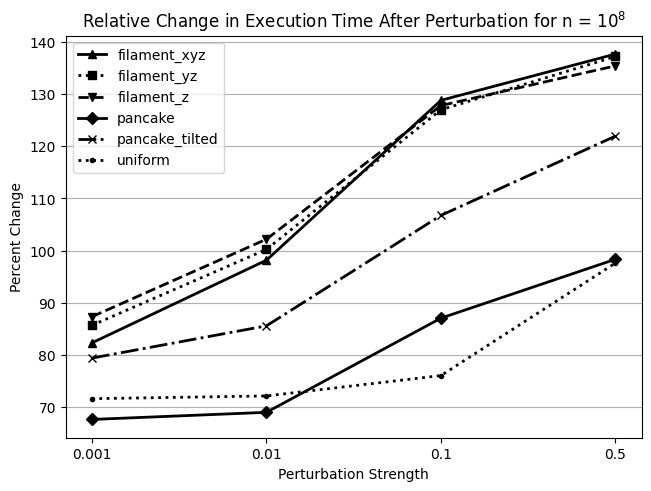
\includegraphics[width=0.45\textwidth]{assets/plotted_n100m.png}
    \caption{Perturbed octree rebalancing time relative to initial build time for different perturbation strengths for a high particle workload of n = $10^8$.}
    \label{fig:plot_100m}
\end{figure}

% Overall in figure \ref{fig:plot_100m} the results were as expected. The general trend shows the rebalancing of the perturbed octree has a dependency on the strength of perturbations. That is as perturbation strength grows time to rebalance grows. What we did not expect to see was that the rebalancing would become significantly greater than even the original build timings, up to $\approx 40\%$ in some cases. This will need to be explored at greater depth in the second half of the project.

% \begin{figure}[h!]
%     \centering
%     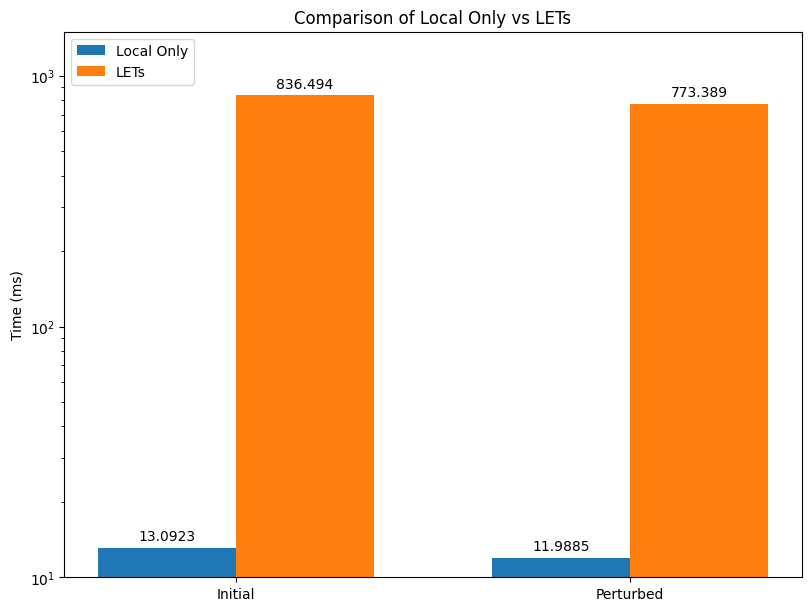
\includegraphics[width=0.45\textwidth]{assets/lets_local_hilbert_10m.png}
%     \caption{Comparison of locally essential tree build time vs. local only using 10 million particles, Hilbert keys, and a uniform distribution using 2 ranks, each with their own GPU.}
%     \label{fig:plot_lets_local}
% \end{figure}

% Figure \ref{fig:plot_lets_local} shows the difference in timing in local octree build times vs. the corresponding times for building the distributed domain for the same number of particles. This shows us the overhead of the distributed case over the single node case. Clearly the overhead is significant at approximately two orders of magnitude in this case. On observation of the profile the largest time sync is the calculation of peer ranks according to the multipole acceptance criterion, this comes as a surprise to us. The operations are all CPU side operations that should incur relatively low latency. We need to gather more data to ensure this is correct and consistent across different sets of hardware. Since it is a CPU side operation the NSight Systems profiler did not pick up much information so getting a perf report should help pickup the issue.

\subsection{Vector Datatypes for Kernel Fusion}
\label{subsec:vd_kf_opt}
The bodies of which the octree is composed of have associated properties. They will of course always $x,y,z$, but they may have more such as mass, charge, and others. The particle SFC keys are sorted during octree construction, which leaves this information inaccessible when traversing the tree. Reordering the properties solves this problem using gather operations on the sorted indexes. These gathers and the sort are by far the most significant bottleneck in local octree construction. 

We achieved significant optimizations in the case of local construction by utilizing vector datatypes and fusing the sort operation with the gathers to sort the vector data. One difference between CPU and GPU programming is that often times it makes more sense to utilize structures of arrays rather than arrays of structures. For example to represent particles in memory on the CPU one might create a struct in C which holds the properties and then create an array of these structures. This makes sense on the CPU because typically a CPU program will access other attributes of the same element after accessing one and this makes for efficient caching. However on a GPU which implements a SIMT model of programming multiple threads in a warp execute the same instructions at the same time. In order to efficiently access global memory with a minimal number of transactions subsequent threads within a warp need to access memory that is contiguous. Typically a structure of arrays makes more sense in this case as the different threads will access the same attribute during the same cycle of the warp. For example if we instead create a particle structure which instead of representing a single particle has arrays for each of its properties an array for $x, y, z$ then when multiple threads access subsequent elements of $x$ they access contiguous memory which then coalesces to a $128-bit$ load or store. For this reason Cornerstone uses arrays to represent the individual particle properties.

Another way to improve bandwidth is to use vector datatypes which allow one to group the properties but still load them efficiently. We utilized this structure instead which allowed us to sort all of the particle properties all at once rather than repeatedly issuing gathers. This ultimately resulted in up to $2.45\times$ improvements in the overall build time of the octree as seen in figure \ref{fig:orig_vs_opt_kt}.

\begin{figure}[h!]
    \centering
    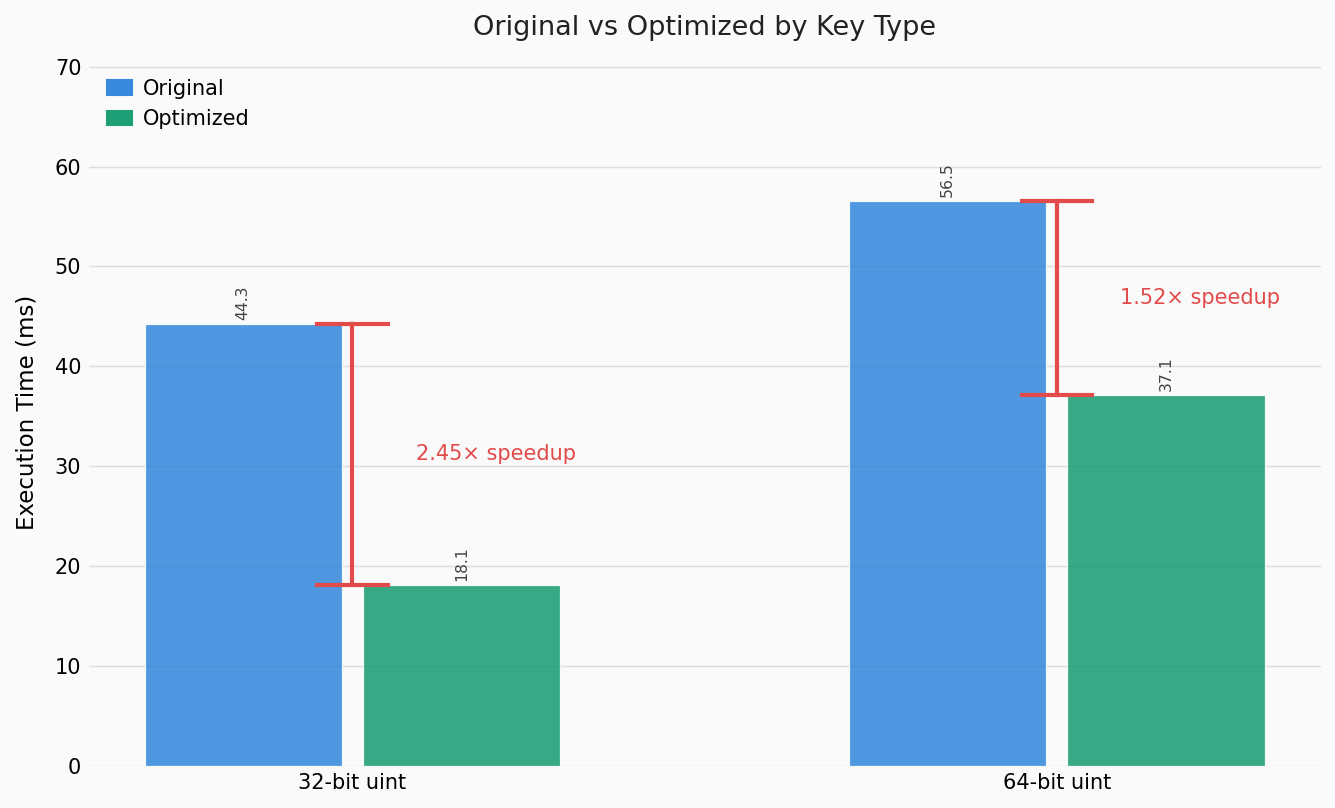
\includegraphics[width=0.45\textwidth]{assets/orig_vs_opt_kt.png}
    \caption{Performance improvements of optimized sort using vector datatypes over original gather for 100m particles on an A100 GPU.}
    \label{fig:orig_vs_opt_kt}
\end{figure}

\subsection{Performance of Local Build vs. GPU Distributed}
\label{subsec:local_dist}

An important aspect of Cornerstone is that it supports distributed processing via domain decomposition and locally essential trees as mentioned in \ref{sec:cornerstone}. We are interested in the overheads associated with building octrees which are partitioned across disaggregated memory modules. This has the benefit of being able to scale out and enables multiple GPUs to work on very large problems that could never fit into a single GPUs memory at once. One difference of note between our work and the problem that Cornerstone ~\cite{cornerstone} is designed to solve is scale, Cornerstone's original purpose is smoothed particle hydrodynamics on exa-scale supercomputers, we are working on a single node on 1-4 GPUs. This difference in scale is likely to expose scalability issues different from the ones the authors needed to consider within the context of their work.

Similarly to the local case, we profiled the distributed method to gauge where bottlenecks were. Figure \ref{fig:dist_flame} shows that a majority of the computation time was spent finding peer ranks, which is a CPU side computation. What is notable is that the communication cost was negligible. This is likely because of the small amount of GPUs tested on because NVLINK was able to greatly lower communication overhead.

\begin{figure*}[t]
    \centering
    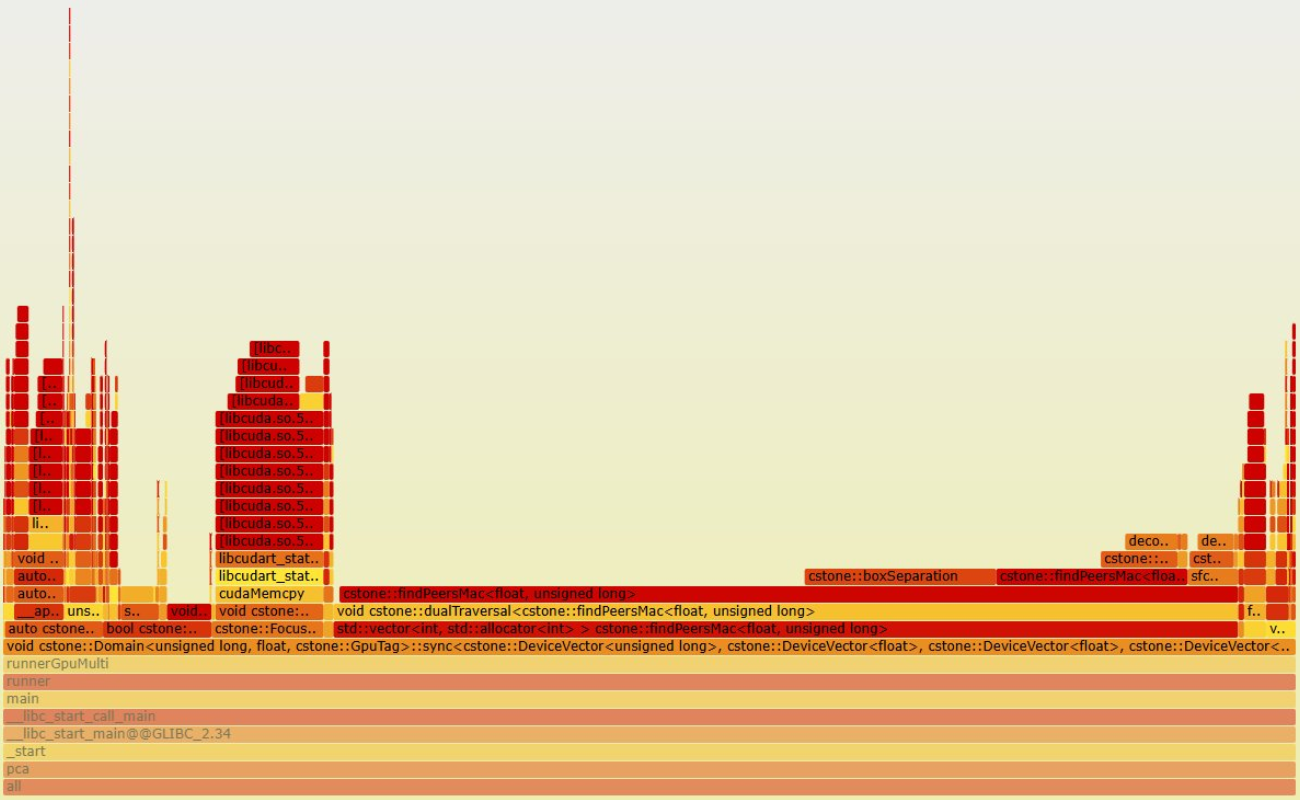
\includegraphics[width=\textwidth]{assets/flame_dist.png}
    \caption{Flame graph profile of distributed construction performance. Finding peers nodes accounts for the largest portion of the computation.}
    \label{fig:dist_flame}
\end{figure*}

We observed the weak scaling of Cornerstone in figure \ref{fig:local_dist} for every combination of configuration options for numbers of particles between 1 million and 100 million; the configuration options included the space filling curve type being either Hilbert or Morton, the number of bits per key being either 32-bits or 64-bits, and the number of GPUs used being either the single GPU local case, or decomposed using 2 or 4 GPUs. In every case the local construction was between 1-2 orders of magnitude faster; this difference in performance is large enough that we can conclude that there is no performance advantage of using distributed construction over local when it is possible to fit the particles on a single GPU. Note that we profile up to the 100 million particles mark, if we were to use the GPU DRAM very well and get within some small factor of filling DRAM we could fit at best, $\frac{TotalDRAM}{sizeof(P)}$ as the number of particles a GPU can support. In the case of an A100 with $40 GB$ of memory and the assumption that a particle consumes $32$ bytes of memory tells us we would be able to fit at most $1,342,177,280$ particles. Such a model is far too optimistic as we will see but this serves to show that even with a very optimistic memory model we are within a factor of 10 of the maximum number of particles a GPU can support which should serve to generalize our conclusion to that there is no performance benefit to using distributed if the number of particles is in this domain. As we can see from figure \ref{fig:local_dist} even with 32 bit Morton keys the local case still beats distributed by roughly an order of magnitude. Given this conclusion the question that drives performance in this regime is at what point the GPUs memory is exhausted and how well we can scale the computation out given the overheads implied by using decomposition.

\begin{figure*}[t]
    \centering
    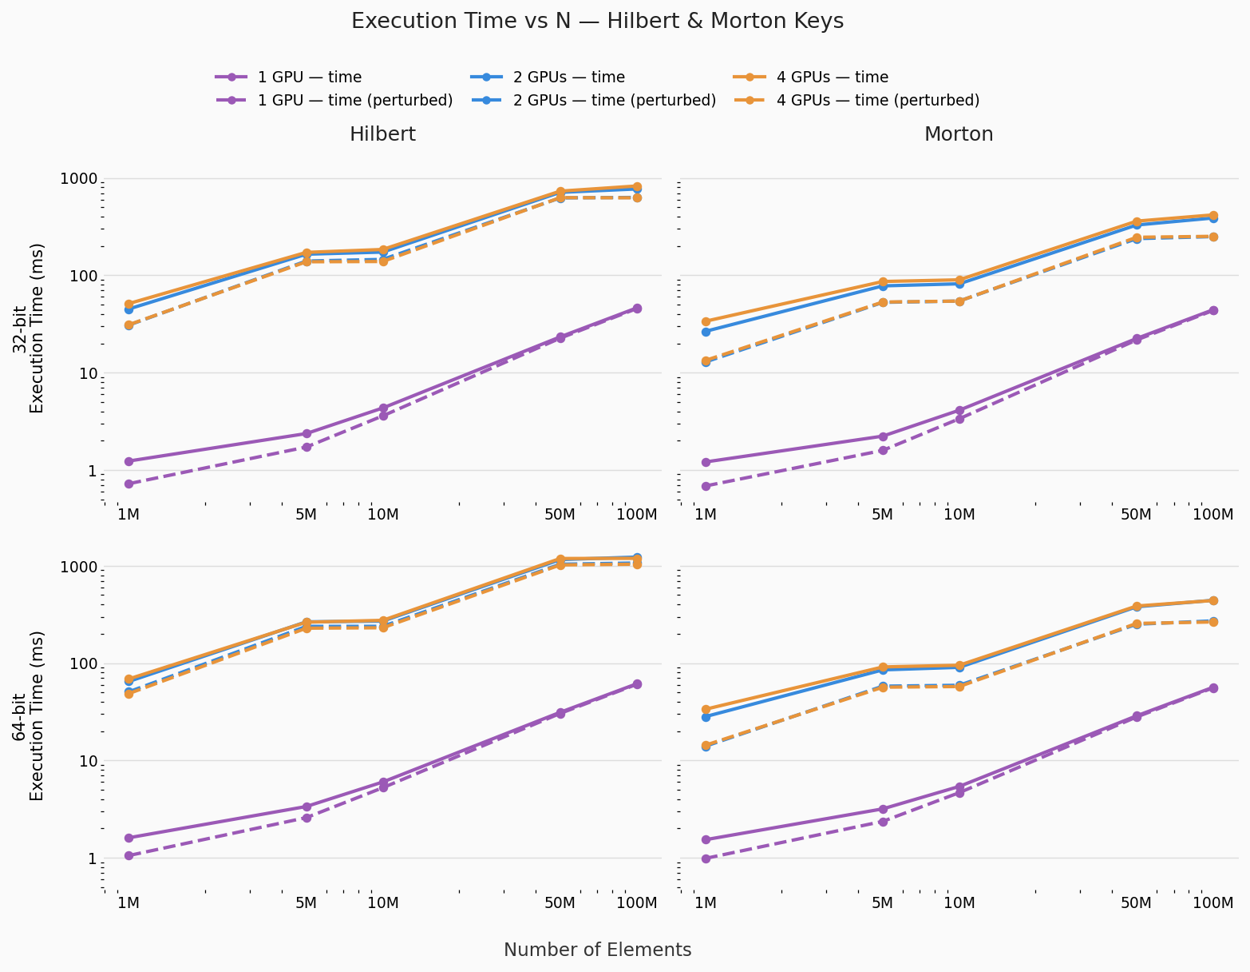
\includegraphics[width=\textwidth]{assets/kbits_ktype_dist_local.png}
    \caption{Performance of different numbers of GPUs across different key configurations on an A100 node.}
    \label{fig:local_dist}
\end{figure*}

We explore the scalability of Cornerstone with respect to memory in figure \ref{fig:mem_comp}. The picture painted by this figure is more concerning, what is clear is that the memory overhead Cornerstone imposes is large enough to be very prohibitive. Given a fixed number of particles on a GPU one might hope that by doubling the number of GPUs, the memory consumed per GPU would roughly split in half since half of the particles would be on the other GPUs. This is clearly not the case, moving from 2 to 4 GPUs gives a much smaller decrease typically between $10\%-20\%$. This has significant implications because to increase the number of particles we require more GPUs to fit them which aside from the performance impacts of needing to use more GPUs one also needs to consider the financial impact of this result. With the total memory being reduced at a rate of roughly $10\%-20\%$ given double the number of GPUs the cost borne to increase capacity is restrictive. 

Digging in to figure \ref{fig:mem_comp} further we see the source of the problem is the overhead of Cornerstone, even though the memory of particles is of course being halved by doubling the number of GPUs, the overhead of Cornerstones internal structures seems to remain quite fixed. Key types had little to no impact on the memory usage but key sizes did noticeably lower memory usage in all cases. It is important to note that there is no data for local construction on 500 million particles as one GPU ran out of memory, with 200 million being the largest particle count we found that could still be constructed locally.

\begin{figure*}[t]
    \centering
    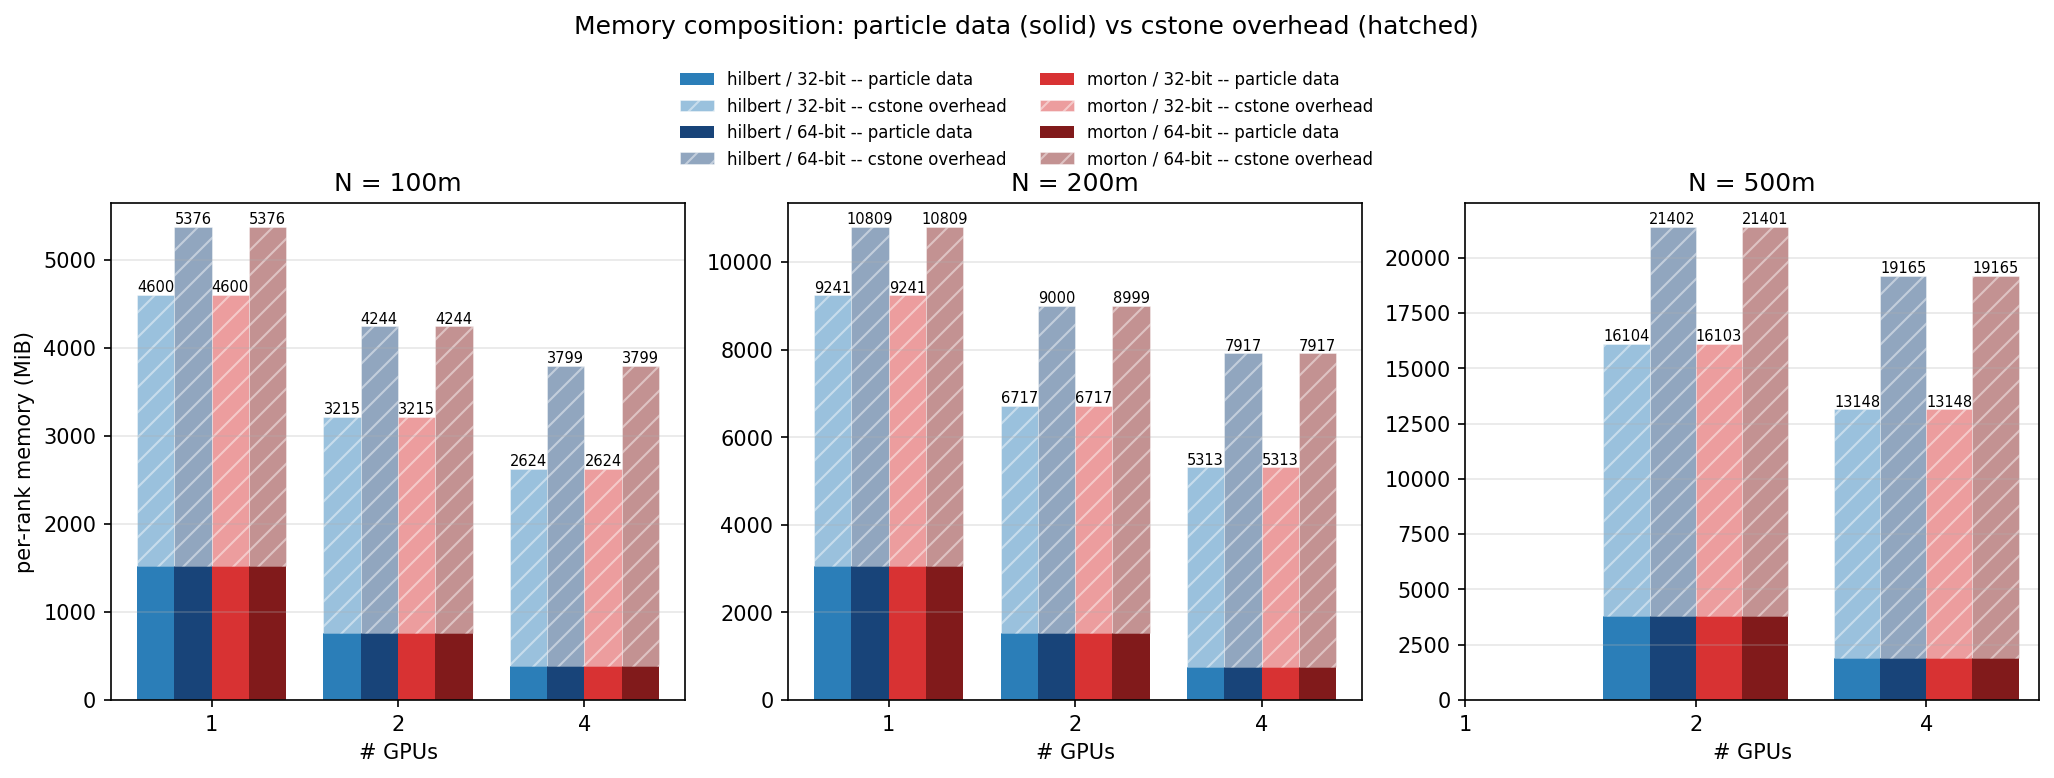
\includegraphics[width=\textwidth]{assets/mem_composition.png}
    \caption{A profile of the memory usage in MiB for varying numbers of GPUs, problem sizes, key bits and types. The chart is divided into a solid region which shows the portion of memory dependent on the particle data and the hatched region which shows the overhead unrelated to the memory consumed by particles specifically; this includes Cornerstone's internal data structures.}
    \label{fig:mem_comp}
\end{figure*}
